% Name: UML state machine
% Description: The life of an order as a UML state machine: an initial and a final state, and transitions labeled event [guard] / action.
% Tags: state machine, UML, state diagram, statechart

\usetikzlibrary{arrows.meta, positioning, calc}

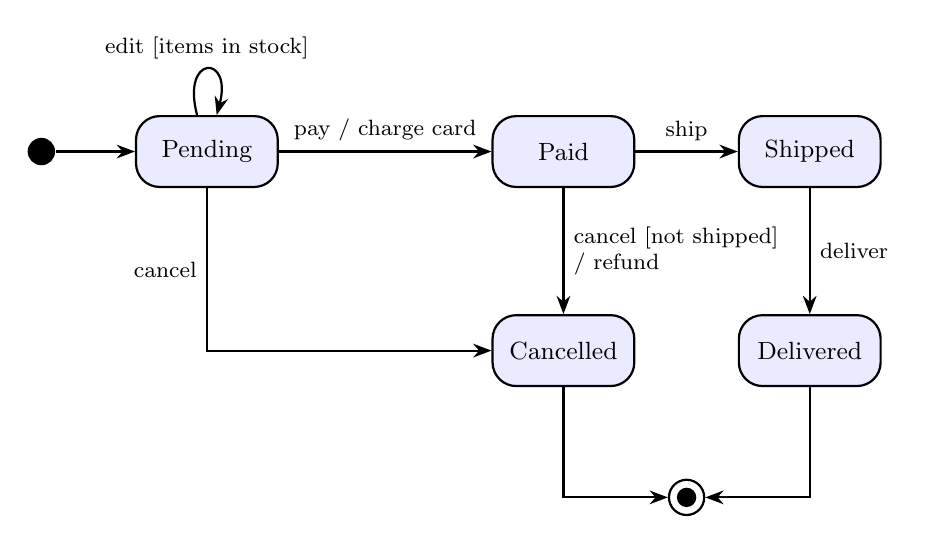
\begin{tikzpicture}[>={Stealth}, thick, node distance=9mm and 13mm, every node/.style={font=\small},
    state/.style={draw, rounded corners=3mm, fill=blue!8, minimum width=18mm, minimum height=9mm},
    label/.style={font=\footnotesize}]
  \node[circle, fill, inner sep=3.5pt] (init) {};
  \node[state, right=10mm of init] (pending) {Pending};
  \node[state, right=27mm of pending] (paid) {Paid};
  \node[state, right=of paid] (shipped) {Shipped};
  \node[state, below=16mm of paid] (cancelled) {Cancelled};
  \node[state, below=16mm of shipped] (delivered) {Delivered};
  \node[circle, draw, inner sep=4.5pt] (final) at ([yshift=-14mm]$(cancelled.south)!0.5!(delivered.south)$) {};
  \fill (final) circle (3.5pt);
  \draw[->] (init) -- (pending);
  \draw[->] (pending) -- node[above, label] {pay / charge card} (paid);
  \draw[->] (paid) -- node[above, label] {ship} (shipped);
  \draw[->] (shipped) -- node[right, label] {deliver} (delivered);
  \draw[->] (pending) |- node[pos=0.25, left, label] {cancel} (cancelled);
  \draw[->] (paid) -- node[right, label, align=left] {cancel [not shipped]\\/ refund} (cancelled);
  \draw[->] (delivered) |- (final);
  \draw[->] (cancelled) |- (final);
  \draw[->] (pending) edge[loop above, min distance=8mm] node[above, label] {edit [items in stock]} (pending);
\end{tikzpicture}
